\newsection
\subsection{BP 1:
  Single wave on a simple beach (Analytic)}

%{\bf Documentation:}  PMEL-135, pp 5 \& 18-30.

\subsubsection{Problems encountered}

\begin{itemize}
\item Numerics for analytical solution to wave equation were hard to determine and should be provided in excel file in description of problem. Analytical solution was obtained from problem champion.
\item No analytical solution given for time $t = 25s$
\item Clawpack code ill suited to computing maximum runup. Additional module needed to be written. 
\end{itemize}

\subsubsection{What we did}

\begin{itemize}
\item Used $g=1$ and no friction.
\item The bathymetry consists of a deep plateau of constant depth $d$ connected to a sloping beach of angle $\beta = arccot(19.85)$. Note that the toe of the beach is located at $x = X_0 = d cot \beta$
\item The initial waveform of the wave is given by 
\begin{equation}
\eta(x,0) = H sech^2(\gamma (x - X_1)/d)
\end{equation}
where $L = arccosh(sqrt(20))/\gamma$, $X_1 = X_0 + L$, and $\gamma = sqrt(3H/4d)$. The speed of the wave is given by the following: 
\begin{equation}
u(x,0)=-\sqrt{g/d}\eta(x,0)
\end{equation}
\item Problem was solved on $800\times 2$ grid, where the x domain spanned from -10 to 60.
\item Variable time stepping was allowed based on a CFL number of 0.9
\end{itemize} 

\subsubsection{Gauge comparisons}
Compare the numerically and analytically computer water level dynamics at locations $x/d = 0.25$ and $x/d = 9.95$ during the propagation and reflection of the wave


See \Fig{bp1gauges}.

\begin{figure}[ht]
\hfil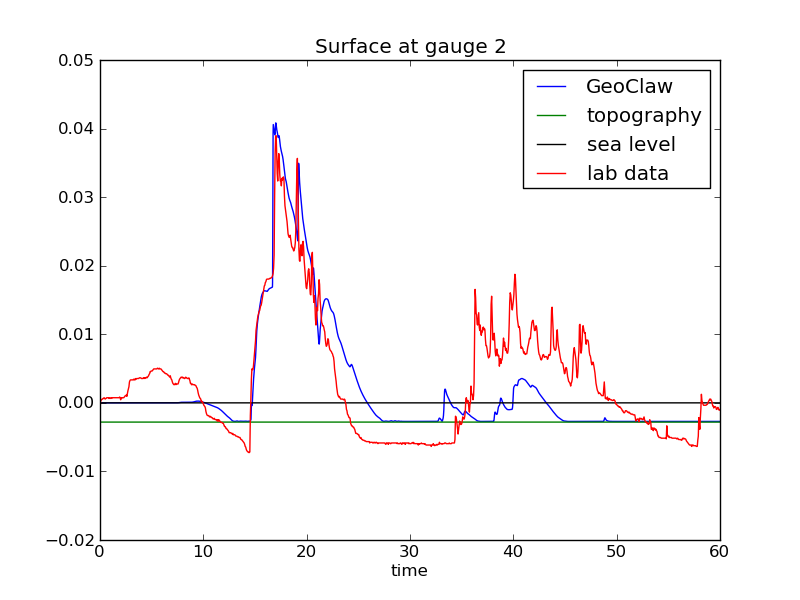
\includegraphics[width=2.8in]{../bp01/canonical-beach/_plots/gauge0002fig300.png}\hfil
\hfil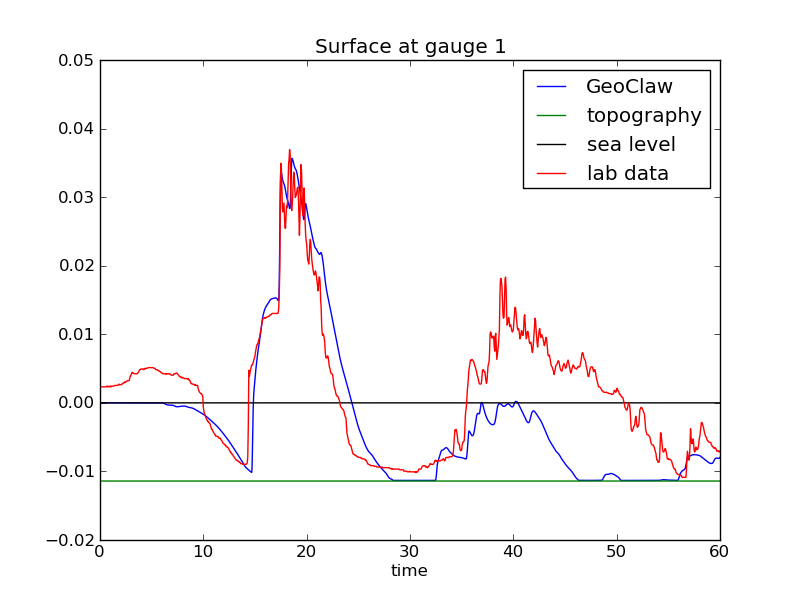
\includegraphics[width=2.8in]{../bp01/canonical-beach/_plots/gauge0001fig300.png}\hfil
\caption{\label{fig:bp1gauges} 
Left column: Gauge profile at location $x/d = 9.95$.
Right column: Gauge profile at location $x/d = 0.25$.
 }
\end{figure}



\subsubsection{Frame comparisons}
Compare the numerically and analytically computed water level profiles at $t = 25(d/g)^{1/2}$, $t = 35(d/g)^{1/2}$, $t = 45(d/g)^{1/2}$, $t = 55(d/g)^{1/2}$, $t = 65(d/g)^{1/2}$.
No analytical solution given for $ t = 25$ ....

See \Fig{bp1frames}
\begin{figure}[ht]
\hfil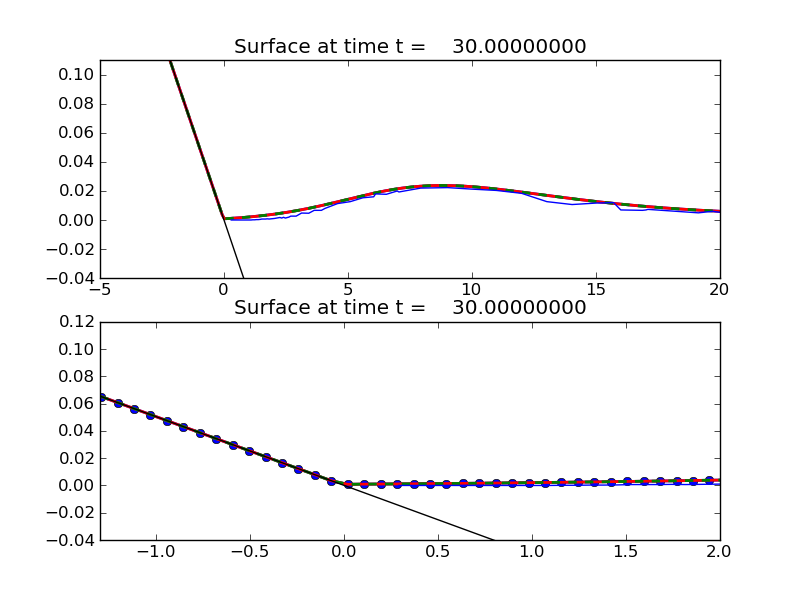
\includegraphics[width=2.8in]{../bp01/canonical-beach/_plots/frame0001fig2.png}\hfil
\hfil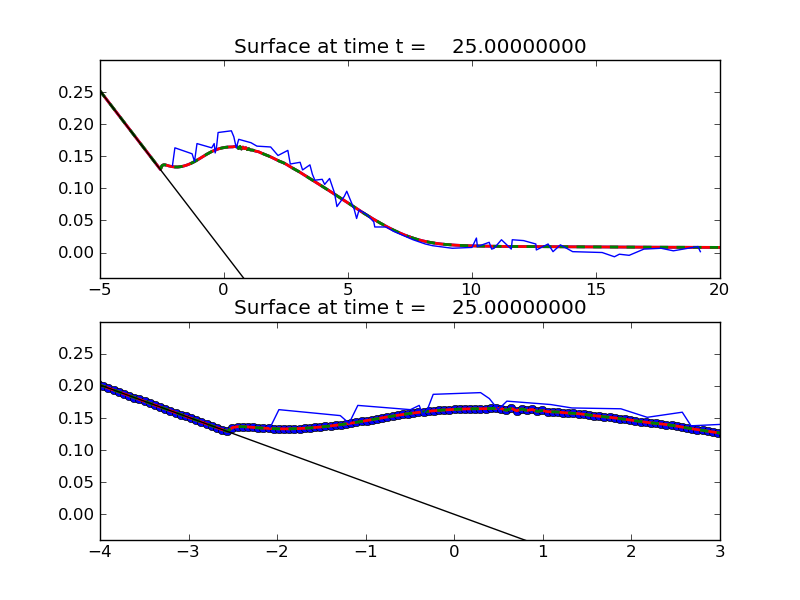
\includegraphics[width=2.8in]{../bp01/canonical-beach/_plots/frame0003fig2.png}\hfil
\vskip 5pt
\hfil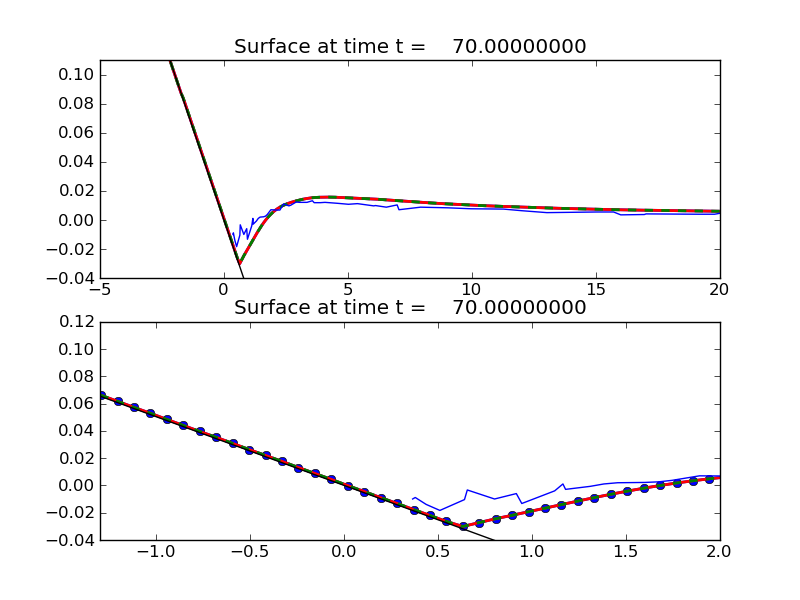
\includegraphics[width=2.8in]{../bp01/canonical-beach/_plots/frame0005fig2.png}\hfil
\hfil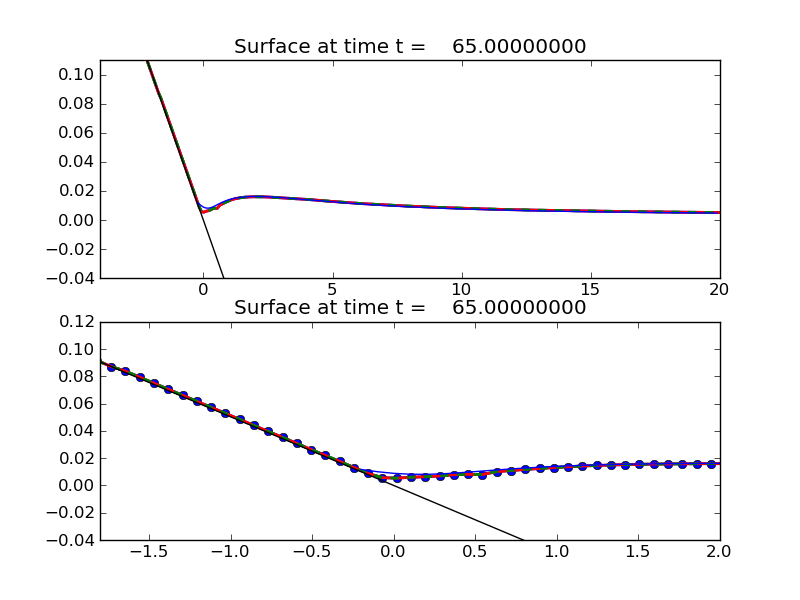
\includegraphics[width=2.8in]{../bp01/canonical-beach/_plots/frame0007fig2.png}\hfil
\caption{\label{fig:bp1frames} 
Frames of runup. Top frame: Full view of incoming wave. Bottom Frame: Zoomed view of inundation area.}
\end{figure}

\subsection{Maximum Runup}
Compute the maximum runup.

\subsection{Lessons learned}

\todo{This was a very relevent benchmark problem because it is a good application of the shallow water wave equations solved analytically in one dimesion. Because the analytical solution is so complex, a numerical solution needs to be provided on the benchmark problem website to ensure all participants are solving the same problem.}
